% Use class option [extendedabs] to prepare the 1-page extended abstract.
\documentclass[extendedabs]{bmvc2k}
\usepackage[colorlinks = true,
            linkcolor = blue,
            urlcolor  = blue,
            citecolor = blue,
            anchorcolor = blue]{hyperref}
\usepackage{kotex} % 한국어 사용 가능

% Document starts here
\begin{document}
\title{기계번역}
\addauthor{
Lee Gwan Hui$^1$, \today}{}{1}
\addinstitution{
$^1$2017142136, Department of Electrical and Electronic Engineering, Yonsei University.}
\maketitle
\let\thefootnote\relax\footnote{This is an extended abstract. The full paper is available at the \href{https://github.com/LeeGwanHui/TIL/tree/main/deeplearning_ham}{github}. }
\vspace{-0.2in}

 \section{GRU\cite{GRU}}
 \subsection{motivation}
 \quad GRU는 RNN의 vanishing gradient problem을 해결할 뿐만 아니라 LSTM에 비해 parameter을 적게 쓰고 cell state도 없다. 따라서 속도가 더 빠르다.

 \subsection{model의 형태\cite{youtube}}
 \quad GRU는 update gate와 reset gate를 활용한다. LSTM의 경우에는 cell state에 어떠한 nonlinear 연산을 하지 않은 반면 
 GRU는 hidden state에 어떠한 nonlinear 연산을 하지 않음으로써 오래된 과거의 정보를 유지할 수 있다. 떄문에 vanishing gradient problem을 해결할 수 있는 것이다.
 전체 구조는 아래와 같다.
 \newline  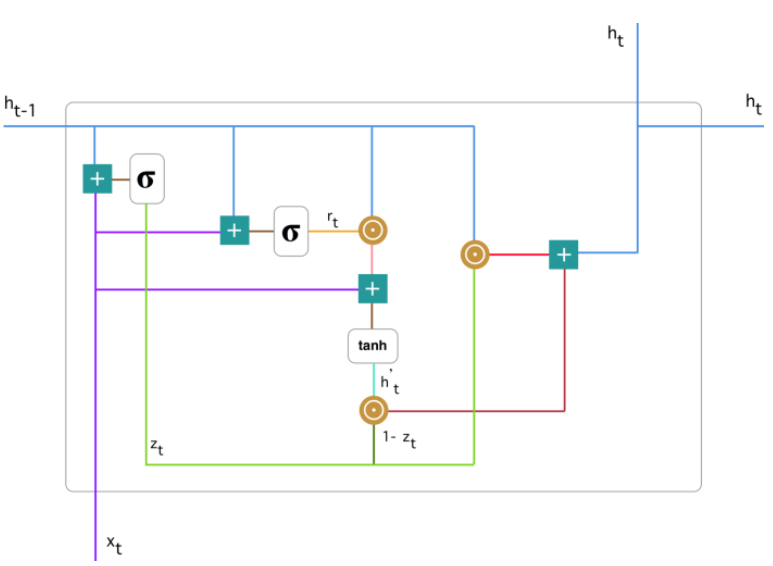
\includegraphics[width=6cm]{images/01_GRU.PNG}
 \newline update gate는 아래와 같은 식으로 계산한다. 
 $$ z_t = \sigma (W^{(z)}x_t + U^{(z)}h_{t-1})$$
 update gate는 과거의 정보를 얼마나 다음 state로 넘겨줄지를 결정한다.
 다음은 reset gate이다. 아래와 같은 식으로 계산한다.
 $$ r_t = \sigma(W^{(r)}x_t + U^{(r)}h_{t-1}) $$
 reset gate에서는 얼마나 과거의 정보를 잊을지를 결정한다. 비슷한 의미라고 생각할 수 있는데 아래 수식을 보자.
 $$ h_t' = tanh(Wx_t + r_t \bigodot U h_{t-1} ) $$
 이렇게 얻은 $r_t$ 의 값을 이용해서 $h_t'$의 값을 계산한다. 이 값은 정보의 관련성을 의미하는 것으로 이 걸로 현재의 정보를 얼마나 저장할지를 결정하게 된다. 
 그리고 이 값과 update gate를 이용해서 아래와 같은 식으로 표현한다.
 $$ h_t = z_t \bigodot h_{t-1} + (1 - z_t) \bigodot h_t'$$
 여기서 $\bigodot$ 은 element wise multiplication을 의미한다. 즉 다시 말해서 $h_t$는 새로운 정보 $(x_t)$ 랑 연산한 결과와 이전 system으로 부터 온 hidden layer output 값을
 얼마나 가중평균을 이용해서 정보를 저장할 건지를 결정하게 된다. 

 \subsection{Conclusion}
 \quad 모델을 보면 $h_t$에는 어떠한 nonlinear 연산이 포함되지 않은 것을 볼 수 있다. 이로써 이 모델은 $h_t$의 정보를 유지하는 것으로 vanishing gradient problem을 해결한 것이다.
 또한 LSTM에 비해서 nonlinear 연산의 수가 줄어들었기 때문에 parameter 수가 감소하였음에도 성능은 차이가 거의 없어서 더 효율적인 모델이다.

 \section{Sequence to Sequence Learning with Neural Network\cite{sutskever2014sequence}}
 \subsection{motivation}
 \quad Deep Neural Network 기법을 사용하여 large labeled training set에서 좋은 성능을 내었다. 하지만 sequence to sequence에서는 사용되지 않았다.
 그 이유로는 기계번역의 특징상 input과 output의 길이가 가변한다는 것이고 이를 해결한 방법이 없었기 때문이다. 이 논문에서는 end-to-end 접근이 가능한
 sequence to sequence model을 제시하는 것을 목표로 한다. 

 \subsection{model의 형태\cite{youtube_seq}}
 \quad 이 논문이 제시한 모델의 기본적인 형태는 encoder과 decoder이다. 먼저 encoder에서 multilayered(4개) LSTM을 사용하여 input sequence을 하나의 고정된 dimensionality를 가지는 vector로 mapping한다.
 그 후 decoder에서 추가적으로 LSTM을 사용해서 vector로 부터 원하는 기계번역에 해당하는 sequence 값을 추출해낸다. 전체적인 그림은 아래와 같다.
 \newline  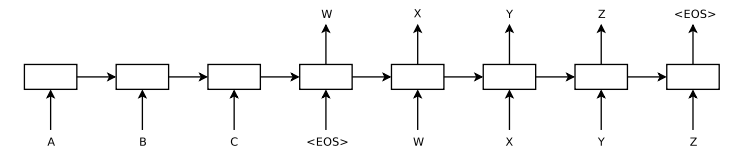
\includegraphics[width=\linewidth]{images/00_seq2seq.PNG}
 먼저 위의 그림을 설명하기 전에 RNN은 input sequence가 주어지면 RNN model을 통과하게 되면 output sequence를 내뱉는다. 아래 식과 같다. 
 $$ h_t = sigmoid(W^{hx}x_t + W^{hh}h_{t-1}) $$
 $$ y_t = W^{yh}h_t $$
 위의 식으로 구하는 것이 RNN의 기본 형태인데 RNN은 long-term dependency 문제에 직면해서 학습이 잘 이루어지지 않는다. 
 이런 단점을 해결하기 위해 나온 모델이 LSTM이다. 이 논문에서는 LSTM을 Recurrent하게 사용하였다. LSTM을 사용할 때 input sequence인 $(x_1, ... , x_T)$ 을 
 fixed dimensional representation vector v로 표현하고(LSTM의 마지막 hidden state의 값 사용), 그 후 새로운 LSTM-LM의 initial hidden state을 v로 사용하고 
 $y_1, ... , y_{T'}$ 을 계산한다.
 $$ p(y_1, ... , y_{T'} | x_1, ... , x_T) = \prod_{t=1}^{T'}p(y_t | v, y_1 , ... , y_{t-1}) $$
 다시 위의 그림으로 돌아가서 설명을 진행해보자. <EOS>는 end-of-sentence symbol를 의미하는 것으 문장의 끝을 표현한다.
 먼저 영어로 표현된 문장을 단어로 분해한 A, B , C 가 있다고 해보자. 이 값을 이제 LSTM에 통과시켜 주면서 마지막 단어인 C가 들어갈 때 나오는 hidden layer의 값은 
 이전의 단어 즉 모든 문장의 정보가 포함되어 있는 vector라고 볼 수 있다. 이 논문의 한계는 이 vector가 고정된 크기라는 것이지만 그럼에도 불구하고 문장을 하나의 고정된 
 vector로 표현해서 문장의 정보를 담고 있는 새로운 data를 만들었다. 이를 이제 다시 LSTM의 hidden layer의 initial 값으로 설정하고 순서대로 값을 추출해주면 X,Y,Z 의 번역된
 sequence를 얻을 수 있다.
 \subsection{Experiments}
 \quad 실험에서는 몇가지 추가적인 방법을 사용하였다. 먼저 첫번째로 encoder과 decoder에서 다른 LSTM을 사용한다. 하나는 input sequence를 위한 것이고 다른 하나는 output sequence를 위한 것이다.
 이렇게 함으로써 model의 parameter을 늘릴 수 있었다고 한다. parameter을 늘리면 느려질 수 있지만 그 만큼 많은 정보를 담고 있을 수 있기 떄문에 언어번역이라는 방대한 양의 data를 다룰때는 좋다.
 두번쨰는 LSTM을 한 층으로 구성한 것이 아니라 four layer로 쌓아서 capacity를 향상시켰다. 이는 위와 같은 이유로 볼 수 있다. 마지막 세번째는 word의 순서를 reverse 시켜서 모델에 넣어주었다는 것인데
 A,B,C를 input 그대로 사용한 것이 아니라 C,B,A 순으로 넣어주었다. 이렇게 함으로써 저자들은 실험적으로 더 좋은 성능을 얻을 수 있었다고 밝힌다. 
 그 이유에 대해서는 영어 문장의 경우에는 주어와 동사가 이어서 나오기 떄문에 문장의 앞의 단어들이 더 연결성이 있는데 문장 그대로 통과시키면 필연적으로 초기에 들어간 단어들은 vanishing이 많이 될 수 밖에 없다.
 그러므로 이를 reverse 시켜주어서 input으로 넣어주는 것이다. 이 같은 구체적인 구조를 적용한 결과 WMT'14 English to French MT task에서 기존의 통계적 방법을 사용한 SMT model이 BLEU 33.3 성능을 보인 반면 
 LSTM으로 만든 모델의 성능은 BLEU 34.8을 달성하였다. 또한 SMT와 LSTM을 같이 사용 했을 떄에는 BLEU 36.5의 성능으로 이 당시 가장 좋은 성능을 가진 모델에 37인 것에 비해 낮지만 충분히 
 기계 번역 task에서도 DNN을 사용할 수 있음을 보였다고 할 수 있다.
 \subsection{Conclusion}
 \quad 이 논문에서는 LSTM을 사용한 seq2seq 모델이 기존의 SMT model 보다 더 좋은 성능을 보임을 밝혔다. 또한 LSTM이 사전에는 긴 문장에 대해서 잘 동작하지 않을 것이라고 생각했음에도 불구하고 매우 성능이 좋았다.
  또한 단순히 input의 순서를 바꿔 주는 것만으로도 성능 향상이 있었다. 가장 중요한 것은 sequence to sequence task에서 DNN의 가능성을 보인 논문이라고 할 수 있다.

 \section{NEURAL MACHINE TRANSLATION BY JOINTLY LEARNING TO ALIGN AND TRANSLATE\cite{bahdanau2014neural}}
 
 \subsection{motivation}
 \quad seq2seq 논문에서 제시한 모델은 input sequence의 정보를 담은 context vector을 만들 때 fixed length vector라는 한계점이 존재했다. 
 즉 가변 길이의 sequence가 들어왔음에도 이를 fixed length vector로 표현했다는 것이다. 이렇게 되면 sentence의 길이가
 길어질수록 성능 저하가 현저히 발생한다. 이 논문에서는 이 문제를 해결한 새로운 모델을 제시한다.
 
 \subsection{model의 형태\cite{youtube_attention}}
 \quad model은 encoder decoder로 구성된다. encoder에서 align과 translation network를 구축한다. 
 이전의 논문인 seq2seq 모델은 긴 문장의 앞부분은 잘 맞더라도 길어지면 뒷부분은 엉망이 되는 문제가 있었다. 그래서 인간이 번역하는 과정 처럼 논문을 번역하는데 어떤 위치의 정보를 번역할 건지 정하자는 것이다.
 즉, 번역을 할때 마지막 hidden state만 사용하는 것이 아니라 모든 hidden state를 적절한 조합으로 만들어내려는 target word와 가장 관련있을법한 곳이 어디인지 찾아보는 network를 추가하자는 것이다.
 이를 이 논문에서는 alignment라고하는데 이 때 attention기법을 사용한다. 이 논문은 attention을 기계번역에 처음 쓴 논문으로 유명하다고 한다.
 제시한 모델은 아래와 같다.
 \newline  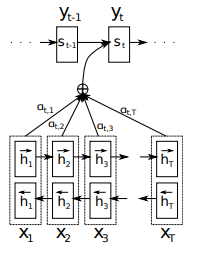
\includegraphics[width=4cm]{images/02_attention.PNG}
 \newline 위의 그림에서 아랫 부분이 encoder이다. encoder은 번역을 할 때 이전에 나온 단어와 함께 앞으로 나올 단어의 정보도 사용하기 위해서 양방향의 RNN을 사용하였다.
 RNN의 구조는 GRU를 사용했다. 식으로 표현하자면 아래와 같다. 
 $$h_j = [ \rightarrow h_j ; \leftarrow h_j]_{concat}$$
 forward 과정에서 얻은 $h_j$ 값과 backward 과정에서 얻은 $h_j$의 값을 concat한 값을 $h_j$로 사용함으로써 목표한 input sequence중의 단어 중에서 $x_i$에 더 초점을 맡춰서 그 주변의 단어들을 볼 수 있게 한다.
 이렇게 얻은 값은 attention에서 사용한다. 위의 모델 그림에서 a가 각 $h_j$ 값을 얼마나 살펴볼 것인지를 결정하는 weight를 의미한다. 아래의 식으로 구한다.
 $$ a_{i,j} = \frac{exp(e_{ij})}{\sum_{k=1}^{T_s} exp(e_{ik})}$$
 위의 a는 e의 값을 softmax한 값이다. 여기서 얻은 a를 가지고 context vector $c_i$를 만들게 된다.
 $$ c_i = \sum_{j=1}^{T_s} a_{ij}h_j $$
 위에 a를 구할 때 e의 값은 아래와 같이 구한다.
 $$ e_{ij} = a(s_{i-1},h_j) $$
 여기서 a는 alignment model을 의미한다. 이 model 역시 학습될 때 함께 학습된다. e의 정확한 식은 아래와 같다.
 $$ e_{ij} = v^T tanh(Ws_{i-1} + V h_j) $$ 
 위의 식을 모두 합쳐서 $c_i$ 을 구할 수 있다. 이렇게 구한 $c_i$ 는 decoder에 사용된다. decoder에서는 $s_i$의 값을 아래와 같이 구한다.
 $$s_i = f(s_{i-1},y_{i-1},c_i)$$
 이렇게 구한 $s_i$ 는 다음 RNN(GRU)에 들어가서 output $y_i$을 추출한다. 여기서 $c_i$ 의 값을 구한다는 것은 index가 있는 것으로 번역하는 단어를 구할 때마다 
 새로 계산한다는 의미이다. 이 때 weight 값인 $a_{i,j}$의 값이 변경된다.

 \subsection{Experiments}
 \quad 기계번역의 대표적인 dataset인  WMT'14 dataset을 이용해서 English to French translation task를 실험했다. 그 결과 아래와 같다.
 \newline  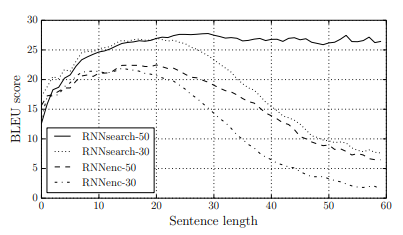
\includegraphics[width=5cm]{images/03_attention.PNG}
 \newline 아래 그림에서 RNNenc는 seq2seq 논문의 model을 의미하고 RNNsearch가 이 논문에서 제시한 모델이다. 본 논문의 model은 문장 길이가 증가해도 성능이 유지가 된다는 것을 볼 수 있다.
 \newline  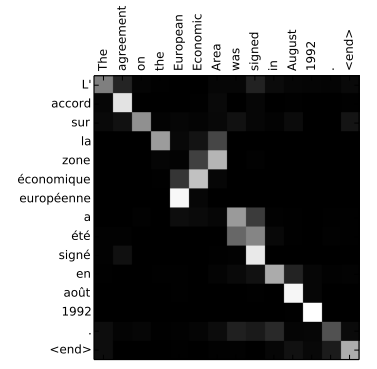
\includegraphics[width=5cm]{images/04_attention.PNG} 
 \newline 위의 결과의 각 pixel은 weight sum 할 때의 계수 크기인 $a_{ij}$을 의미한다. x축은 input sentence를 y축은 output sentence를 의미한다. 이 결과를 보면 번역 결과를 나타낼 때 적절한 
 위치의 단어를 더 충실히 보고 결과를 도출해낸 것을 알 수 있다.
 
 \subsection{Conclusion}
 \quad seq2seq의 fixed-length context vector의 한계를 개선하는 새로운 encoder-decoder approach를 제시하였다. encoder에서는 양방향의 RNN을 사용해서 input sequence의 target word의
 앞의 단어 뿐만 아니라 다음 단어도 볼 수 있음을 적절히 이용했고 또한 alignment model을 구현해서 번역하고자하는 input sequence의 위치를 찾고 이를 attention 기법으로 구현하였다. 
 제안한 model이 seq2seq model의 fixed context vector을 해결하여 긴 문장에서도 더 좋은 성능을 보였다.


\newpage
\bibliography{egbib}

\end{document}